\documentclass[UTF8,a4paper,12pt]{ctexart}

\usepackage{geometry}
\usepackage{graphicx}
\usepackage{float}
\usepackage{booktabs}
\usepackage{longtable}
\usepackage{array}
\usepackage{amsmath}
\usepackage{amssymb}
\usepackage{xcolor}
\usepackage{listings}
\usepackage{hyperref}
\usepackage{caption}
\usepackage{subcaption}
\usepackage{tikz}
\usetikzlibrary{positioning}
\graphicspath{{figures/}}

\geometry{left=2.5cm,right=2.5cm,top=2.6cm,bottom=2.6cm}
\setlength{\parindent}{2em}
\setlength{\parskip}{0.25em}
\linespread{1.25}

\hypersetup{
  colorlinks=true,
  linkcolor=black,
  urlcolor=blue,
  citecolor=black
}

\lstset{
  basicstyle=\ttfamily\small,
  keywordstyle=\color{blue!70!black},
  commentstyle=\color{green!40!black},
  stringstyle=\color{red!60!black},
  numbers=left,
  numberstyle=\tiny\color{gray},
  frame=single,
  breaklines=true,
  tabsize=4,
  showstringspaces=false,
  columns=fullflexible
}

\newcommand{\placeholderfigure}[2]{
  \begin{figure}[H]
    \centering
    \begin{tikzpicture}
      \draw[gray, thick, dashed] (0,0) rectangle (12,5.5);
      \node[align=center, text=gray!80!black] at (6,2.75)
      {#1\\[0.6em]\small 建议补充文件：\path{#2}};
    \end{tikzpicture}
    \caption{#1（待补充）}
  \end{figure}
}

\newcommand{\maybeimage}[3]{
  \IfFileExists{#2}{
    \begin{figure}[H]
      \centering
      \includegraphics[width=0.88\textwidth]{#2}
      \caption{#1}
    \end{figure}
  }{
    \placeholderfigure{#1}{#2}
  }
}

\title{\textbf{基于视觉迷宫识别的五自由度机械臂绘制系统实验报告}}
\author{项目名称：Maze 机械臂迷宫绘制系统}
\date{\today}

\begin{document}

\maketitle

\begin{abstract}
本实验围绕 ``让机械臂根据摄像头拍摄的纸面迷宫自动规划路径并完成描绘'' 这一目标，完成了图像重建、路径规划、机械臂运动学求解、仿真验证和真实机械臂控制的完整系统。系统输入为一张白纸黑笔绘制的迷宫照片，其中红色标记起点、蓝色标记终点；程序首先对纸面进行透视矫正和二值化重建，再基于占用栅格执行 A* 路径搜索，最后将二维路径转换为五自由度机械臂关节轨迹，并通过 TCP 与串口链路下发给真实机械臂。实验表明，本项目能够形成从照片输入到机械臂描绘输出的闭环流程，体现了视觉处理、搜索算法、机器人运动学和上下位机通信的综合应用。
\end{abstract}

\tableofcontents
\newpage

\section{实验概述}

本项目的核心任务是将普通摄像头拍摄到的 ``白纸黑笔迷宫'' 转换为机械臂可以执行的绘图轨迹。迷宫照片存在拍摄角度倾斜、光照不均和背景干扰等问题，因此系统需要先完成图像重建；之后在迷宫通道中规划从起点到终点的路径；最后将路径转换为真实纸面上的物理坐标，并通过逆运动学求出机械臂五个关节的角度指令。

\begin{figure}[H]
  \centering
  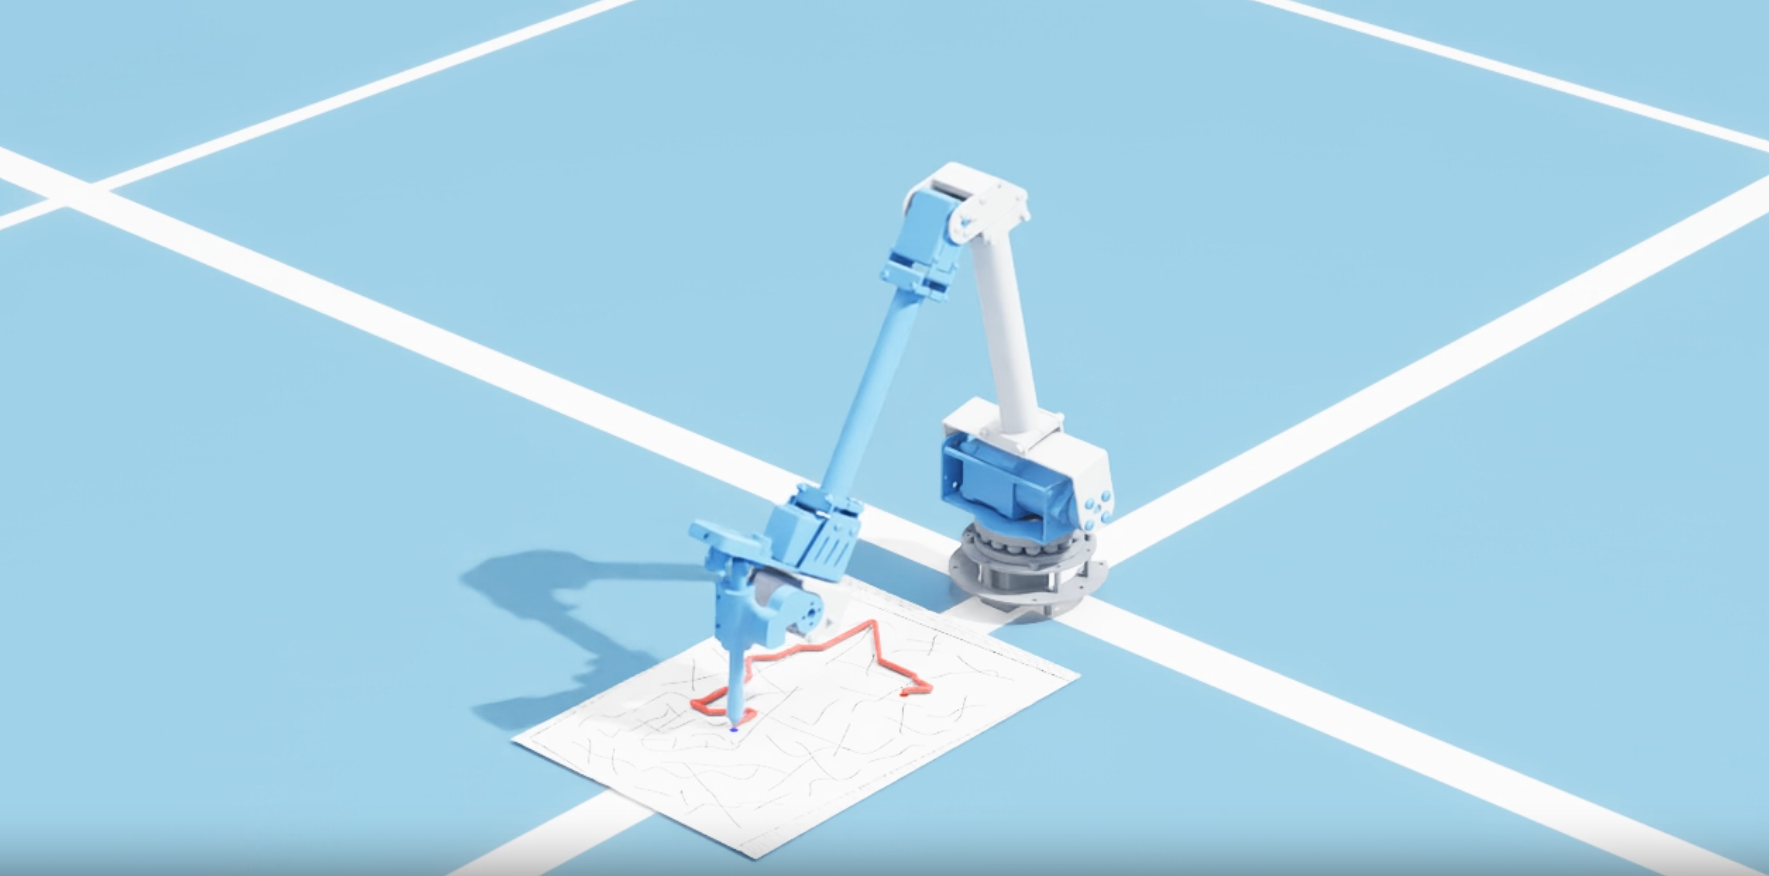
\includegraphics[width=0.88\textwidth]{overview.png}
  \caption{项目总体效果图}
\end{figure}

系统分为四个主要层次，如表 \ref{tab:modules} 所示。

\begin{table}[H]
  \centering
  \caption{系统模块划分}
  \label{tab:modules}
  \begin{tabular}{p{3cm}p{6cm}p{5cm}}
    \toprule
    模块 & 功能 & 对应代码 \\
    \midrule
    视觉重建 & 从倾斜拍摄照片中恢复正视图和黑白扫描图 & \texttt{maze\_planner/maze\_scanner.py} \\
    路径规划 & 检测红色起点、蓝色终点，基于占用栅格执行 A* 搜索 & \texttt{maze\_planner/maze\_planner.py} \\
    仿真验证 & 在 Isaac Sim 中导入 5-DOF 机械臂并验证绘图过程 & \texttt{arm\_sim/draw\_maze.py} \\
    实机执行 & 将轨迹转换为关节角，通过 TCP 与串口控制真实机械臂 & \texttt{arm\_real\_client/}、\texttt{arm\_real\_server/} \\
    \bottomrule
  \end{tabular}
\end{table}

\section{硬件与软件平台}

\subsection{硬件平台}

实验使用一台五自由度桌面机械臂。机械臂末端原夹爪位置被改装为固定笔的连接件，使末端能够作为绘图笔在纸面上运动。机械臂通过 USB 串口与下位机 Windows 主机通信，并需要外接 12V 电源供电。

\maybeimage{真实机械臂整体搭建照片}{figures/real_setup.jpg}{}
\maybeimage{末端笔固定结构近景}{figures/pen_mount.jpg}{}

机械臂的 URDF 模型位于 \texttt{urdf/five\_dof\_arm.urdf}，对应的 STL 网格文件存放在 \texttt{urdf/meshes/}。仿真中使用的零位姿态和可达区域如图 \ref{fig:zero_pose}、图 \ref{fig:reachable} 所示。

\begin{figure}[H]
  \centering
  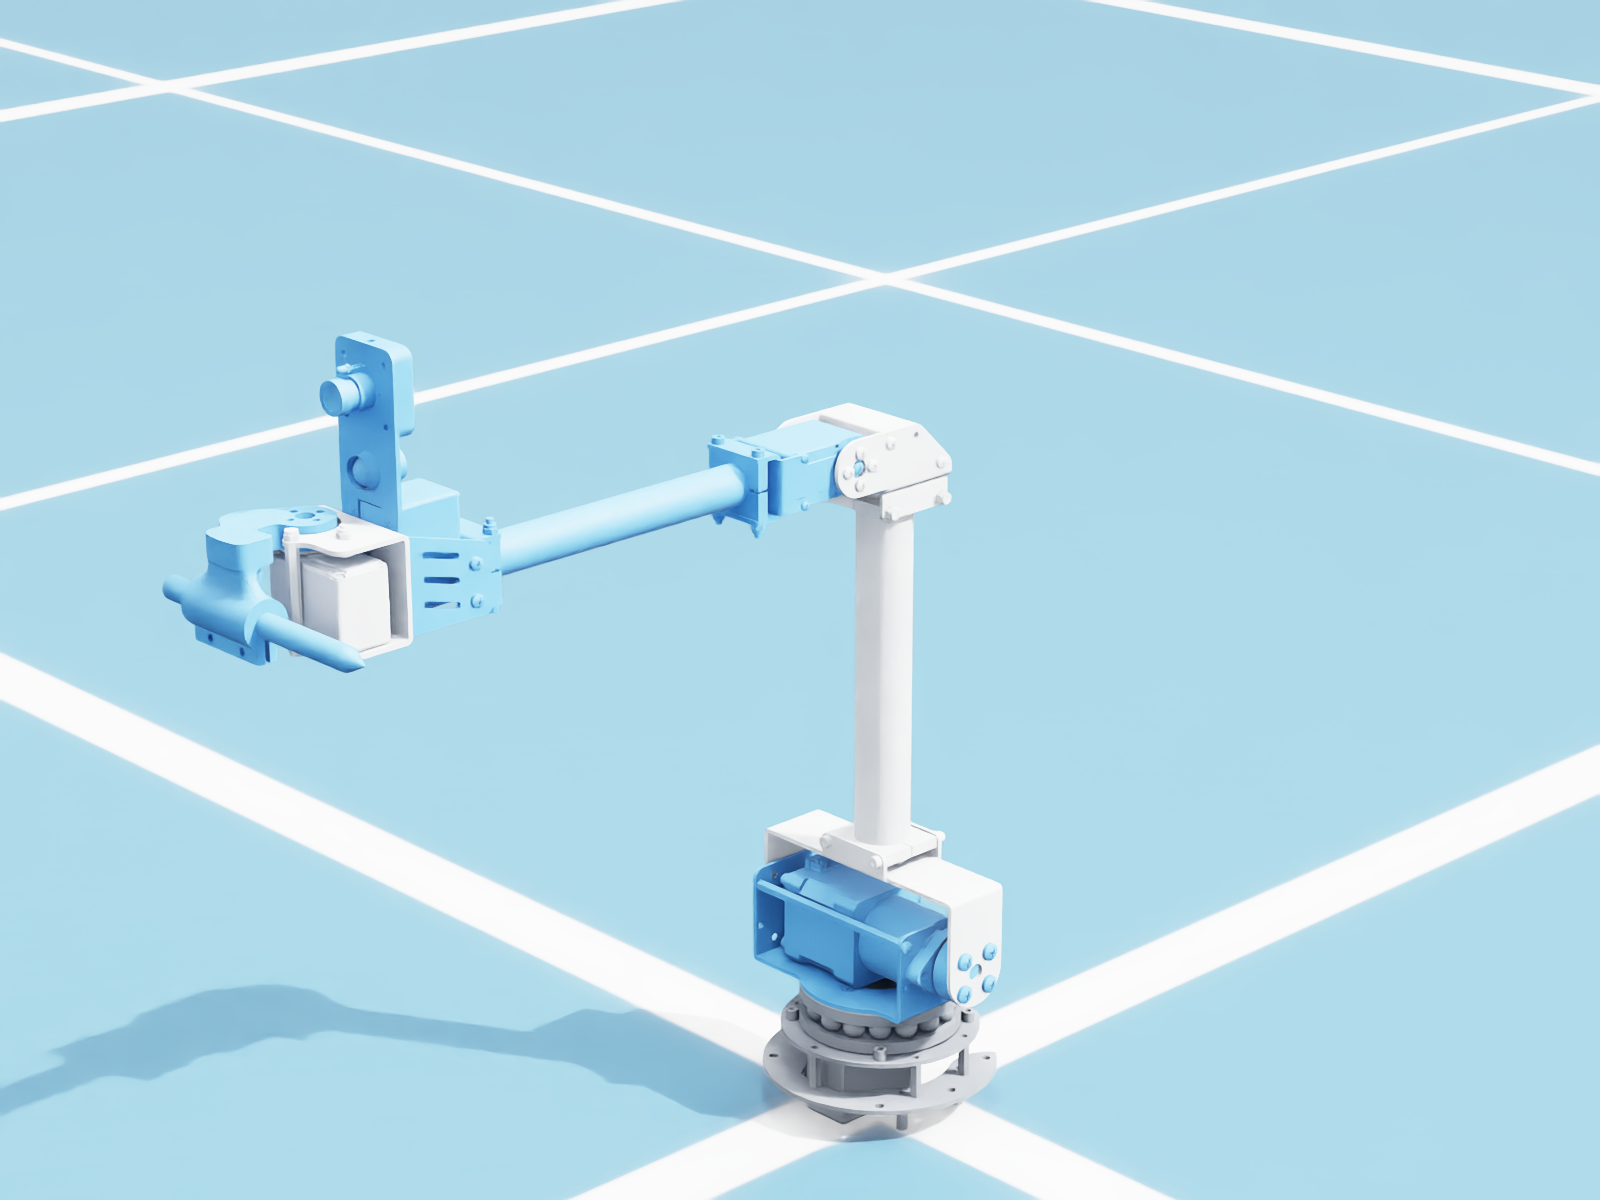
\includegraphics[width=0.72\textwidth]{zero_pose.png}
  \caption{机械臂零位姿态}
  \label{fig:zero_pose}
\end{figure}

\begin{figure}[H]
  \centering
  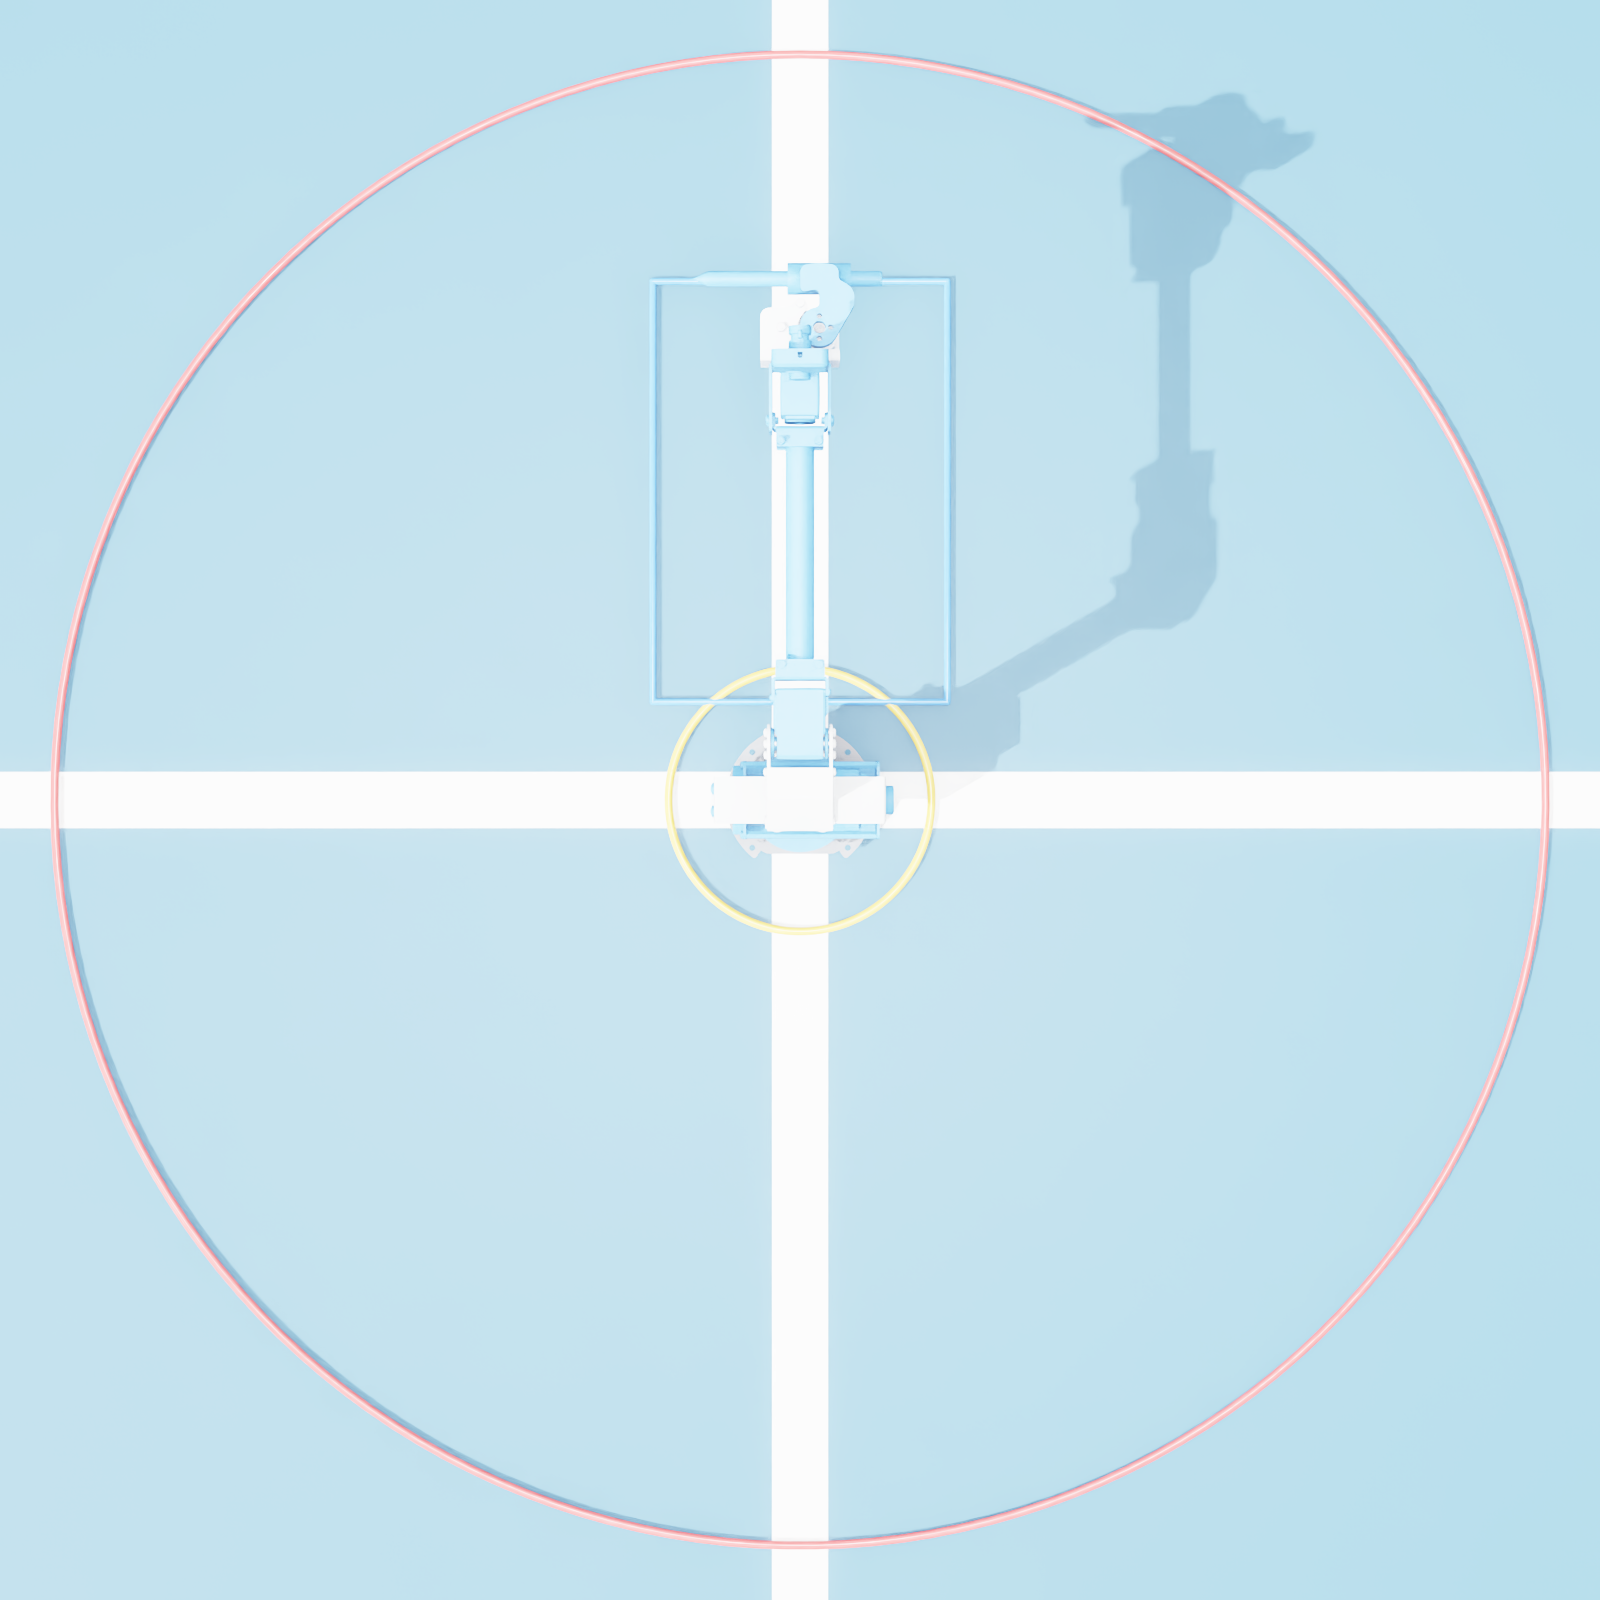
\includegraphics[width=0.72\textwidth]{reachable_area.png}
  \caption{机械臂可达空间}
  \label{fig:reachable}
\end{figure}

\subsection{软件平台}

项目主要使用 Python 实现，核心依赖包括 OpenCV、NumPy、SciPy、Isaac Sim、socket 和 pyserial。其中 OpenCV 用于纸面检测、透视变换、二值化和颜色标记检测；NumPy 与 SciPy 用于坐标变换、轨迹重采样和逆运动学优化；Isaac Sim 用于机械臂仿真与视频渲染；socket 与 pyserial 用于真实机械臂控制链路。

项目中的 \texttt{maze\_planner/environment.yml} 用于创建迷宫识别和规划环境。Isaac Sim 仿真需要单独配置带 GPU 渲染能力的环境。

\section{系统总体方案}

系统从照片输入到真实机械臂执行的整体流程如图 \ref{fig:pipeline} 所示。

\begin{figure}[H]
  \centering
  \begin{tikzpicture}[
    node distance=0.9cm and 0.9cm,
    box/.style={draw, rounded corners, align=center, minimum height=0.85cm, minimum width=2.45cm},
    arrow/.style={->, thick}
  ]
    \node[box] (a) {迷宫照片};
    \node[box, right=of a] (b) {透视矫正\\二值化};
    \node[box, right=of b] (c) {占用栅格\\A*规划};
    \node[box, below=of c] (d) {路径重采样\\坐标映射};
    \node[box, left=of d] (e) {逆运动学\\关节轨迹};
    \node[box, left=of e] (f) {仿真验证\\实机下发};
    \draw[arrow] (a) -- (b);
    \draw[arrow] (b) -- (c);
    \draw[arrow] (c) -- (d);
    \draw[arrow] (d) -- (e);
    \draw[arrow] (e) -- (f);
  \end{tikzpicture}
  \caption{系统总体流程}
  \label{fig:pipeline}
\end{figure}

系统采用模块化设计。视觉和路径规划模块只负责生成像素路径；仿真和实机模块共享同一套图像坐标到世界坐标的映射函数，并复用 \texttt{arm\_kinematics.py} 中的运动学求解逻辑，从而保证仿真轨迹与实机轨迹的一致性。

\section{项目结构与模块关系}

本项目并不是单一脚本，而是按照 ``感知--规划--运动学--仿真--实机控制'' 的机器人系统链路组织。仓库中各目录职责如下：

\begin{lstlisting}[language=bash, caption={项目主要目录结构}]
Maze/
  maze_planner/          # 迷宫视觉重建与路径规划
    maze_scanner.py      # 纸面检测、透视矫正、增强、二值化
    maze_planner.py      # 起终点检测、占用栅格、A* 路径搜索
    samples/             # 测试迷宫照片
    outputs/             # 中间图、规划结果、关节轨迹

  arm_sim/               # Isaac Sim 仿真与运动学验证
    arm_kinematics.py    # 5-DOF 正运动学、逆运动学
    draw_maze.py         # 将规划路径转换为仿真绘制动作
    draw_circle.py       # 画圆验证 FK/IK 链路
    video/               # 仿真渲染视频

  arm_real_client/       # 上位机：规划、IK、轨迹下发
    draw_maze_real.py    # 图片 -> 路径 -> 关节轨迹 -> TCP 下发
    robot_client.py      # TCP JSON 客户端封装
    estop.py             # 软件停止后续轨迹下发

  arm_real_server/       # 下位机：TCP 服务与串口控制
    robot_server.py      # 接收轨迹、限位、逐点执行、状态反馈
    robot_server_openloop.py # 开环定时执行版本，便于对比调试

  urdf/                  # 机械臂模型文件
    five_dof_arm.urdf
    meshes/

  assets/                # 项目展示图与仿真截图
\end{lstlisting}

从数据流角度看，\texttt{maze\_planner} 产生的是图像路径点；\texttt{arm\_sim} 与 \texttt{arm\_real\_client} 都会调用 \texttt{arm\_kinematics.py} 将路径点转换为关节角；\texttt{arm\_real\_server} 不再参与路径规划，而是专注于硬件通信、限位保护和轨迹执行。模块关系如图 \ref{fig:module_relation} 所示。

\begin{figure}[H]
  \centering
  \begin{tikzpicture}[
    node distance=0.8cm and 1.1cm,
    box/.style={draw, rounded corners, align=center, minimum height=0.9cm, minimum width=3.2cm},
    arrow/.style={->, thick}
  ]
    \node[box] (scanner) {\texttt{maze\_scanner}\\照片重建};
    \node[box, right=of scanner] (planner) {\texttt{maze\_planner}\\A* 路径规划};
    \node[box, right=of planner] (kin) {\texttt{arm\_kinematics}\\FK/IK 求解};
    \node[box, below left=of kin] (sim) {\texttt{arm\_sim}\\仿真验证};
    \node[box, below right=of kin] (client) {\texttt{arm\_real\_client}\\轨迹生成/下发};
    \node[box, below=of client] (server) {\texttt{arm\_real\_server}\\串口执行/反馈};
    \draw[arrow] (scanner) -- node[above]{二值图/矫正图} (planner);
    \draw[arrow] (planner) -- node[above]{像素路径} (kin);
    \draw[arrow] (kin) -- node[left]{关节轨迹} (sim);
    \draw[arrow] (kin) -- node[right]{关节轨迹 JSON} (client);
    \draw[arrow] (client) -- node[right]{TCP JSON} (server);
  \end{tikzpicture}
  \caption{项目模块关系}
  \label{fig:module_relation}
\end{figure}

\section{迷宫图像重建}

\subsection{纸面检测与透视矫正}

摄像头拍摄的迷宫照片通常存在倾斜、透视畸变、阴影和背景干扰。程序首先通过亮度与饱和度特征检测白纸区域；若检测失败，则退化到 Canny 边缘检测。得到纸面四个角点后，程序按左上、右上、右下、左下排序，并执行透视变换，将倾斜纸面恢复为正视图。

\begin{lstlisting}[language=Python, caption={四点透视矫正核心代码}]
def four_point_transform(img, rect):
    tl, tr, br, bl = rect
    width_top = np.linalg.norm(tr - tl)
    width_bottom = np.linalg.norm(br - bl)
    height_left = np.linalg.norm(bl - tl)
    height_right = np.linalg.norm(br - tr)
    max_w = int(round(max(width_top, width_bottom)))
    max_h = int(round(max(height_left, height_right)))

    dst = np.array([[0, 0],
                    [max_w - 1, 0],
                    [max_w - 1, max_h - 1],
                    [0, max_h - 1]], dtype="float32")
    M = cv2.getPerspectiveTransform(rect, dst)
    return cv2.warpPerspective(img, M, (max_w, max_h))
\end{lstlisting}

\begin{figure}[H]
  \centering
  
\includegraphics[width=0.72\textwidth]{1_paper_detected.png}
  \caption{纸面检测结果}
\end{figure}

\begin{figure}[H]
  \centering
  
\includegraphics[width=0.72\textwidth]{2_warped.png}
  \caption{透视矫正后的迷宫图像}
\end{figure}

\subsection{亮度增强与二值化}

为了降低光照不均和阴影对识别的影响，程序使用大尺度高斯模糊估计背景，再将原图除以背景实现光照归一化，随后使用 CLAHE 增强局部对比度。最后通过自适应阈值得到黑白扫描图。

\begin{lstlisting}[language=Python, caption={亮度增强核心代码}]
def enhance(img):
    gray = cv2.cvtColor(img, cv2.COLOR_BGR2GRAY) if img.ndim == 3 else img
    k = max(31, (max(gray.shape) // 20) | 1)
    background = cv2.GaussianBlur(gray, (k, k), 0)
    background = np.where(background == 0, 1, background)
    norm = gray.astype(np.float32) / background.astype(np.float32)
    norm = np.clip(norm, 0, 1)
    norm = (norm * 255).astype(np.uint8)
    clahe = cv2.createCLAHE(clipLimit=2.0, tileGridSize=(8, 8))
    return clahe.apply(norm)
\end{lstlisting}

\begin{figure}[H]
  \centering
  \begin{subfigure}{0.48\textwidth}
    \centering
    
\includegraphics[width=\textwidth]{3_enhanced.png}
    \caption{亮度增强结果}
  \end{subfigure}
  \hfill
  \begin{subfigure}{0.48\textwidth}
    \centering
    
\includegraphics[width=\textwidth]{4_binary.png}
    \caption{二值化结果}
  \end{subfigure}
  \caption{图像增强与二值化中间结果}
\end{figure}

经过连通域过滤和形态学清理后，得到更适合路径规划的扫描图，如图 \ref{fig:scan_result} 所示。

\begin{figure}[H]
  \centering
  
\includegraphics[width=0.72\textwidth]{5_result.png}
  \caption{清理后的黑白扫描图}
  \label{fig:scan_result}
\end{figure}

\section{路径规划算法}

\subsection{规划问题数学描述}

迷宫路径规划可以抽象为二维栅格地图上的最短路搜索问题。设透视矫正后的二值图像尺寸为 $W \times H$，像素点为
\[
  p=(x,y), \quad 0 \le x < W,\ 0 \le y < H .
\]
根据二值扫描图构造占用函数
\[
  O(x,y)=
  \begin{cases}
    1, & I(x,y)<128,\ \text{该点属于墙体或障碍};\\
    0, & I(x,y)\ge 128,\ \text{该点属于可通行区域}.
  \end{cases}
\]
为了提高搜索效率，程序将像素级地图降采样为最大边长不超过 \texttt{grid\_max} 的栅格地图。若缩放比例为
\[
  s=\frac{\texttt{grid\_max}}{\max(W,H)},
\]
则像素坐标 $p=(x,y)$ 映射到栅格坐标
\[
  c=(r,c)=\left(\left\lfloor sy \right\rceil,\left\lfloor sx \right\rceil\right).
\]
搜索图可以表示为
\[
  G=(V,E), \quad
  V=\{(r,c)\mid O_g(r,c)=0\},
\]
其中 $O_g$ 为降采样并膨胀后的占用栅格。边集合 $E$ 采用 8 邻接，水平和竖直移动代价为 $1$，对角移动代价为 $\sqrt{2}$。规划目标是在起点 $c_s$ 与终点 $c_g$ 之间寻找总代价最小的路径
\[
  P^*=\arg\min_P \sum_{i=1}^{n-1} w(c_i,c_{i+1}),
  \quad c_1=c_s,\ c_n=c_g .
\]

\subsection{起点与终点检测}

路径规划模块从透视矫正后的彩色图中检测颜色标记：红色区域作为起点，蓝色区域作为终点。程序将图像转换到 HSV 空间，对红色和蓝色分别设置阈值，并取最大连通域质心作为标记中心。

\begin{lstlisting}[language=Python, caption={红蓝标记检测代码}]
def detect_markers(bgr):
    hsv = cv2.cvtColor(bgr, cv2.COLOR_BGR2HSV)
    k = np.ones((5, 5), np.uint8)

    red = cv2.inRange(hsv, (0, 80, 40), (10, 255, 255)) | \
          cv2.inRange(hsv, (170, 80, 40), (180, 255, 255))
    red = cv2.morphologyEx(red, cv2.MORPH_OPEN, k)

    blue = cv2.inRange(hsv, (100, 80, 40), (130, 255, 255))
    blue = cv2.morphologyEx(blue, cv2.MORPH_OPEN, k)
    return _largest_blob_centroid(red), _largest_blob_centroid(blue)
\end{lstlisting}

\subsection{占用栅格构建}

黑色笔迹代表迷宫墙体，白色区域代表可通行区域。程序先将二值图转为墙体栅格，再擦除起终点附近的颜色标记，随后通过闭运算修补墙体断缝，并对墙体进行膨胀，为笔尖尺寸和运动误差预留安全距离。

墙体膨胀在机器人学中相当于把点机器人规划转化为考虑机器人半径的配置空间规划。设机械臂末端笔尖和执行误差需要预留的安全半径为 $\rho$ 个栅格，则膨胀后的障碍集合为
\[
  \mathcal{O}_{\mathrm{inflated}}
  = \mathcal{O} \oplus B_{\rho},
\]
其中 $\oplus$ 表示 Minkowski 和，$B_{\rho}$ 为半径 $\rho$ 的结构元素。代码中用 OpenCV 的 \texttt{dilate} 实现这一操作。

\begin{lstlisting}[language=Python, caption={占用栅格构建核心代码}]
def build_occupancy(binary, markers, close=5, inflate=1, grid_max=400):
    h0, w0 = binary.shape
    wall = (binary < 128).astype(np.uint8)

    erase_r = max(12, int(0.02 * max(h0, w0)))
    for m in markers:
        if m is not None:
            cv2.circle(wall, (int(round(m[0])), int(round(m[1]))),
                       erase_r, 0, -1)

    if close > 0:
        wall = cv2.morphologyEx(wall, cv2.MORPH_CLOSE,
                                np.ones((close, close), np.uint8))
    scale = grid_max / float(max(h0, w0))
    if scale < 1.0:
        gh, gw = max(int(h0 * scale), 1), max(int(w0 * scale), 1)
        wall = (cv2.resize(wall * 255, (gw, gh),
                           interpolation=cv2.INTER_AREA) > 0).astype(np.uint8)
    else:
        scale = 1.0
    if inflate > 0:
        wall = cv2.dilate(wall, np.ones((2 * inflate + 1,) * 2, np.uint8))
    return wall.astype(bool), scale
\end{lstlisting}

\begin{figure}[H]
  \centering
  
\includegraphics[width=0.72\textwidth]{6_occupancy.png}
  \caption{占用栅格结果：白色为可走区域，黑色为障碍区域}
\end{figure}

\subsection{A* 搜索}

本项目使用 8 邻接 A* 算法搜索从起点到终点的最短可行路径。直行代价为 1，对角移动代价为 1.414，启发函数采用欧氏距离。为了避免路径从两堵墙之间的对角缝隙中穿过，程序在对角移动时额外检查相邻正交格是否同时为障碍。

A* 对每个候选节点 $n$ 维护评价函数
\[
  f(n)=g(n)+h(n),
\]
其中 $g(n)$ 是从起点到当前节点的累计代价，$h(n)$ 是到终点的启发式估计。本项目使用欧氏距离作为启发函数：
\[
  h(n)=\sqrt{(r_n-r_g)^2+(c_n-c_g)^2}.
\]
由于欧氏距离不会高估 8 邻接栅格中的真实最短代价，因此该启发函数是 admissible 的，能够保证 A* 在离散栅格图上找到最优路径。代码中的 \texttt{gscore} 保存 $g(n)$，\texttt{open\_heap} 按 $f(n)$ 从小到大弹出候选节点，\texttt{came} 保存父节点用于回溯路径。

\begin{lstlisting}[language=Python, caption={A* 搜索中的邻域扩展与对角穿墙检查}]
for dr, dc, cost in nbrs:
    nr, nc = cr + dr, cc + dc
    if not (0 <= nr < h and 0 <= nc < w) or occ[nr, nc]:
        continue
    if dr != 0 and dc != 0 and (occ[cr + dr, cc] and occ[cr, cc + dc]):
        continue
    ng = g + cost
    if ng < gscore.get((nr, nc), float("inf")):
        gscore[(nr, nc)] = ng
        came[(nr, nc)] = cur
        heapq.heappush(open_heap, (ng + heur((nr, nc), goal), ng, (nr, nc)))
\end{lstlisting}

最终路径规划结果如图 \ref{fig:planned} 所示，紫色线条为机械臂将要描绘的路径。

\begin{figure}[H]
  \centering
  
\includegraphics[width=0.75\textwidth]{planned.png}
  \caption{规划路径叠加图}
  \label{fig:planned}
\end{figure}

\section{机械臂运动学与轨迹生成}

\subsection{像素坐标到纸面坐标的映射}

图像路径点首先按弧长重采样，保证轨迹点分布均匀。随后将矫正图像中的像素坐标映射到真实纸面的物理坐标。项目中纸面尺寸设置为 $30\ \mathrm{cm} \times 21\ \mathrm{cm}$，纸面中心相对机械臂底座的位置由 \texttt{paper\_cx} 与 \texttt{paper\_cy} 控制。

设矫正图像坐标为 $(p_x,p_y)$，图像宽高为 $(W,H)$，归一化纹理坐标为
\[
  u=\frac{p_x}{W}, \qquad v=\frac{p_y}{H}.
\]
纸面中心在机械臂基坐标系下的位置为 $(x_c,y_c,z_{\mathrm{paper}})$，纸张沿 $x$ 与 $y$ 方向的尺寸分别为 $L_x=0.30\ \mathrm{m}$、$L_y=0.21\ \mathrm{m}$。因此目标笔尖坐标定义为
\[
  \mathbf{x}_d =
  \begin{bmatrix}
    x_c + (0.5-v)L_x \\
    y_c + (u-0.5)L_y \\
    z_{\mathrm{paper}} + \Delta z
  \end{bmatrix},
\]
其中 $\Delta z=0.001\ \mathrm{m}$，用于让笔尖略高于纸面模型，便于仿真和实机落笔调节。

\begin{lstlisting}[language=Python, caption={图像坐标到纸面世界坐标的映射}]
PAPER_SX, PAPER_SY, PAPER_TOP = 0.30, 0.21, 0.002
PEN_Z = PAPER_TOP + 0.001

def img_to_world(px, py, wimg, himg, paper_cx, paper_cy):
    u, v = px / wimg, py / himg
    return (paper_cx + (0.5 - v) * PAPER_SX,
            paper_cy + (u - 0.5) * PAPER_SY, PEN_Z)
\end{lstlisting}

该映射同时用于仿真脚本 \texttt{arm\_sim/draw\_maze.py} 和实机脚本 \texttt{arm\_real\_client/draw\_maze\_real.py}，因此仿真中看到的纸面轨迹与真实下发轨迹保持一致。

\subsection{路径弧长重采样}

A* 输出的路径是栅格折线，点间距会随栅格搜索方向变化。若直接把这些格点下发给机械臂，会导致局部速度不均匀，转弯处也可能出现轨迹点过密或过疏。为此，程序按折线弧长进行等距重采样。

设规划得到的像素路径为
\[
  P=\{\mathbf{p}_0,\mathbf{p}_1,\ldots,\mathbf{p}_{m-1}\},
\]
累计弧长为
\[
  l_0=0,\qquad
  l_i=\sum_{k=1}^{i}\left\|\mathbf{p}_k-\mathbf{p}_{k-1}\right\|_2 .
\]
若希望生成 $N$ 个机械臂轨迹点，则在 $[0,l_{m-1}]$ 上均匀采样
\[
  \hat{l}_j=\frac{j}{N-1}l_{m-1},\qquad j=0,1,\ldots,N-1,
\]
并对 $x$、$y$ 坐标分别做一维线性插值，得到等弧长路径点 $\hat{\mathbf{p}}_j$。

\begin{lstlisting}[language=Python, caption={路径弧长重采样代码}]
def resample(pts, n):
    P = np.asarray(pts, float)
    d = np.r_[0, np.cumsum(np.linalg.norm(np.diff(P, axis=0), axis=1))]
    s = np.linspace(0, d[-1], n)
    return np.c_[np.interp(s, d, P[:, 0]), np.interp(s, d, P[:, 1])]
\end{lstlisting}

\subsection{正运动学}

\texttt{arm\_kinematics.py} 按 URDF 中定义的关节 origin、rpy 和 axis 建立五个关节的齐次变换链。通过逐级矩阵相乘，可以得到末端 link\_5 的位姿，再根据笔尖在 link\_5 坐标系下的偏移求出世界坐标中的笔尖位置。

设五个关节角为
\[
  \mathbf{q}=[q_1,q_2,q_3,q_4,q_5]^T .
\]
第 $i$ 个关节由 URDF 中的固定平移 $\mathbf{t}_i$、固定姿态 $R_i^{0}$ 和绕关节轴的旋转 $R_z(\sigma_i q_i)$ 组成，其中 $\sigma_i\in\{-1,1\}$ 表示 URDF 轴方向与程序角度正方向的关系。因此单关节齐次变换可写为
\[
  {}^{i-1}T_i(\mathbf{q})=
  \begin{bmatrix}
    R_i^{0}R_z(\sigma_i q_i) & \mathbf{t}_i\\
    \mathbf{0}^T & 1
  \end{bmatrix}.
\]
末端 link\_5 相对基坐标系的位姿为
\[
  {}^{0}T_5(\mathbf{q})=
  \prod_{i=1}^{5} {}^{i-1}T_i(q_i).
\]
若笔尖在 link\_5 坐标系下的坐标为 ${}^{5}\mathbf{p}_{nib}$，则世界坐标中的笔尖位置为
\[
  {}^{0}\mathbf{p}_{nib} =
  {}^{0}R_5(\mathbf{q})\,{}^{5}\mathbf{p}_{nib}
  +{}^{0}\mathbf{t}_5(\mathbf{q}).
\]

\begin{lstlisting}[language=Python, caption={五自由度机械臂正运动学}]
def fk_M5(q):
    M = np.eye(4)
    for (tr, rot, sign), th in zip(_JOINTS, q):
        M = M @ tr @ rot @ _Rz(sign * th)
    return M

def fk_nib_tail(q):
    M5 = fk_M5(q)
    o, R = M5[:3, 3], M5[:3, :3]
    return o + R @ _NIB, o + R @ _TAIL
\end{lstlisting}

从机器人学角度看，也可以定义笔尖位置雅可比
\[
  J_p(\mathbf{q})=
  \frac{\partial\,{}^{0}\mathbf{p}_{nib}}{\partial \mathbf{q}}
  \in \mathbb{R}^{3\times 5}.
\]
不过当前分支的实现并不显式构造雅可比矩阵，而是直接将正运动学函数作为非线性优化目标交给 SciPy 的 SLSQP 求解器处理。这样代码更短，也便于把真实机械臂的关节限位直接作为优化边界加入。

\subsection{逆运动学}

逆运动学求解使用 SciPy 的 SLSQP 有界优化。求解目标分为两个优先级：首先保证笔尖位置到达目标点；若目标点在关节限位内可达，则在保持笔尖位置的约束下优化笔轴方向，使笔尽量竖直向下。

第一阶段只优化位置误差：
\[
  \mathbf{q}_{pos} =
  \arg\min_{\mathbf{q}_{min}\le \mathbf{q}\le \mathbf{q}_{max}}
  \left\| \mathbf{p}_{nib}(\mathbf{q})-\mathbf{x}_d \right\|_2^2 .
\]
若最小位置误差仍大于阈值，说明该目标点在当前关节限位和纸面摆放下不可达，程序直接返回最接近的关节解并报告残差。若位置可达，则进入第二阶段，在保持笔尖位置不变的条件下优化笔轴姿态。

设笔尖点为 $\mathbf{p}_{nib}$、笔尾点为 $\mathbf{p}_{tail}$，则笔轴单位向量为
\[
  \mathbf{a}(\mathbf{q})=
  \frac{\mathbf{p}_{nib}(\mathbf{q})-\mathbf{p}_{tail}(\mathbf{q})}
       {\left\|\mathbf{p}_{nib}(\mathbf{q})-\mathbf{p}_{tail}(\mathbf{q})\right\|_2}.
\]
理想绘图姿态为笔轴竖直向下，即 $\mathbf{a}_d=[0,0,-1]^T$。第二阶段优化目标可写为
\[
  \mathbf{q}^{*} =
  \arg\min_{\mathbf{q}_{min}\le \mathbf{q}\le \mathbf{q}_{max}}
  \left(1+a_z(\mathbf{q})\right)
  + \lambda \left\|\mathbf{q}-\mathbf{q}_{ref}\right\|_2^2,
\]
\[
  \mathrm{s.t.}\quad
  \mathbf{p}_{nib}(\mathbf{q})=\mathbf{x}_d .
\]
其中 $1+a_z$ 在笔轴越接近竖直向下时越小，$\lambda \left\|\mathbf{q}-\mathbf{q}_{ref}\right\|_2^2$ 是连续性正则项，用于避免相邻轨迹点之间关节角跳变过大。

\begin{lstlisting}[language=Python, caption={逆运动学优化框架}]
def ik(target, q0, lim=None):
    del lim  # 旧接口兼容；实际限位固定为真机可动范围。
    target = np.asarray(target, float)
    q_ref = np.clip(np.asarray(q0, float), _JOINT_LO, _JOINT_HI)

    def pos_cost(q):
        err = fk_pos(q) - target
        return float(err @ err)

    pos_res = minimize(pos_cost, q_ref, method="SLSQP", bounds=_BOUNDS)
    q_pos = np.clip(pos_res.x if pos_res.x is not None else q_ref,
                    _JOINT_LO, _JOINT_HI)
    pos_err = float(np.linalg.norm(fk_pos(q_pos) - target))

    if pos_err > _POS_TOL:
        a = _pen_axis(q_pos)
        tilt = np.degrees(np.arccos(np.clip(-a[2], -1, 1)))
        return q_pos, pos_err, float(tilt)

    def orient_cost(q):
        a = _pen_axis(q)
        return float((1.0 + a[2]) + _CONTINUITY_W * np.sum((q - q_ref) ** 2))

    orient_res = minimize(orient_cost, q_pos, method="SLSQP",
                          bounds=_BOUNDS,
                          constraints=({"type": "eq",
                                        "fun": lambda q: fk_pos(q) - target},))
    q = np.clip(orient_res.x if orient_res.x is not None else q_pos,
                _JOINT_LO, _JOINT_HI)
    if np.linalg.norm(fk_pos(q) - target) > max(_POS_TOL, pos_err * 2.0):
        q = q_pos
    a = _pen_axis(q)
    tilt = np.degrees(np.arccos(np.clip(-a[2], -1, 1)))
    return q, float(np.linalg.norm(fk_pos(q) - target)), float(tilt)
\end{lstlisting}

真实机械臂执行时，\texttt{draw\_maze\_real.py} 会沿路径逐点调用 IK，并将弧度制关节角转换为舵机指令角度：
\[
  \boldsymbol{\theta}_{deg}=\frac{180}{\pi}\mathbf{q}.
\]
随后按 URDF 关节顺序映射到真机控制字段
\[
  [q_1,q_2,q_3,q_4,q_5] \longrightarrow [b,s,e,w,h],
\]
并在下发前检查各关节是否满足机械臂限位。当前分支中，第 5 关节 $h$ 虽然已经由夹爪改装为笔旋转关节，但真实可动范围仍按 $\pm45^\circ$ 处理；腕关节 $w$ 按 $\pm90^\circ$ 保守限位。因此 IK 中的边界为
\[
  \mathbf{q}_{min}=[-180,-90,-90,-90,-45]^\circ,\quad
  \mathbf{q}_{max}=[180,90,90,90,45]^\circ .
\]

当前轨迹文件 \texttt{maze\_planner/outputs/trajectory/trajectory.json} 中保存了 70 个轨迹点，其元信息如表 \ref{tab:traj_meta} 所示。

\begin{table}[H]
  \centering
  \caption{轨迹文件元信息}
  \label{tab:traj_meta}
  \begin{tabular}{ll}
    \toprule
    指标 & 数值 \\
    \midrule
    输入图片 & \texttt{maze\_planner/samples/test\_0.jpg} \\
    轨迹点数 & 70 \\
    纸面中心距底座 & \texttt{paper\_cx = 0.22 m} \\
    点间时间 & \texttt{dt = 0.1 s} \\
    最大 IK 位置残差 & 约 $0.0494$ mm \\
    最大笔轴偏离竖直角 & 约 $0.572^\circ$ \\
    \bottomrule
  \end{tabular}
\end{table}

\section{Isaac Sim 仿真验证}

仿真模块将机械臂 URDF 导入 Isaac Sim，并把重建后的迷宫图作为纸面纹理贴到 $30\ \mathrm{cm} \times 21\ \mathrm{cm}$ 的平面上。程序逐点设置机械臂关节角，同时用红色轨迹点显示笔尖已走过的路径，最后渲染为 MP4 视频。

\begin{lstlisting}[language=Python, caption={仿真中路径到关节轨迹的转换}]
pts, warped, binary, start_xy, goal_xy = solve_path(MAZE_IMG, auto=True,
                                                    debug_dir=_IMG_DIR)
path_px = resample(pts, N_WAYPOINTS)
targets = [img_to_world(px, py, wimg, himg) for px, py in path_px]

qtraj, res, tilt = [], [], []
q_seed = np.array([0.0, 1.0, 1.0, 0.0, 0.0])
for tgt in targets:
    q_seed, e, ti = ik(np.array(tgt), q_seed)
    qtraj.append(q_seed.copy())
    res.append(e)
    tilt.append(ti)
\end{lstlisting}

仿真输出文件包括 \texttt{arm\_sim/video/arm\_motion.mp4}、\texttt{arm\_sim/video/arm\_draw\_circle.mp4} 和 \texttt{arm\_sim/video/arm\_draw\_maze.mp4}。其中 \texttt{arm\_draw\_maze.mp4} 展示了机械臂沿迷宫规划路径描绘的完整过程。

\maybeimage{Isaac Sim 中机械臂描绘迷宫关键帧}{figures/sim_draw_maze_frame.jpg}{}

\section{真实机械臂控制实现}

\subsection{上下位机通信链路}

真实机械臂控制采用 ``上位机规划 + 下位机执行'' 的结构。上位机负责图像处理、路径规划、IK 求解和轨迹文件生成；下位机运行在 Windows 上，直接通过 pyserial 访问机械臂串口，并对上位机开放 TCP 服务。

\begin{figure}[H]
  \centering
  \begin{tikzpicture}[
    node distance=0.7cm,
    box/.style={draw, rounded corners, align=center, minimum height=0.9cm, minimum width=7.8cm},
    arrow/.style={->, thick}
  ]
    \node[box] (a) {上位机：\texttt{draw\_maze\_real.py / robot\_client.py}};
    \node[box, below=of a] (b) {TCP JSON 通信：端口 9001};
    \node[box, below=of b] (c) {下位机：\texttt{robot\_server.py}};
    \node[box, below=of c] (d) {pyserial 串口：COM4/环境变量 @ 115200};
    \node[box, below=of d] (e) {机械臂主控板};
    \draw[arrow] (a) -- (b);
    \draw[arrow] (b) -- (c);
    \draw[arrow] (c) -- (d);
    \draw[arrow] (d) -- (e);
  \end{tikzpicture}
  \caption{上下位机通信链路}
\end{figure}

\texttt{robot\_client.py} 将所有请求封装为一行 JSON，通过 TCP 发送给服务器。

\begin{lstlisting}[language=Python, caption={上位机轨迹下发接口}]
class RobotClient:
    def request(self, payload):
        msg = json.dumps(payload, separators=(",", ":")) + "\n"
        with socket.create_connection((self.host, self.port),
                                      timeout=self.timeout) as sock:
            sock.sendall(msg.encode("utf-8"))
            data = sock.recv(4096)
        return json.loads(data.decode("utf-8"))

    def trajectory(self, points, dt=DEFAULT_DT, traj_id="traj",
                   spd=DEFAULT_SPD, acc=DEFAULT_ACC):
        return self.request({
            "type": "trajectory",
            "traj_id": traj_id,
            "dt": dt,
            "spd": spd,
            "acc": acc,
            "points": points,
        })
\end{lstlisting}

\subsection{下位机串口指令}

下位机服务端将上位机传来的关节角转换为机械臂底层 JSON 串口协议。关节控制指令使用 \texttt{T=122}，包括底座 \texttt{b}、肩关节 \texttt{s}、肘关节 \texttt{e}、腕关节 \texttt{w} 和末端 \texttt{h}，并附带速度与加速度。

当前分支的下位机默认监听 \texttt{0.0.0.0:9001}，串口默认为 Windows 下的 \texttt{COM4}，也可以通过环境变量 \texttt{ROBOT\_SERIAL\_PORT}、\texttt{ROBOT\_SERVER\_HOST} 和 \texttt{ROBOT\_SERVER\_PORT} 覆盖。相比旧的 WSL 中转方案，当前实现由 \texttt{robot\_server.py} 一个进程同时完成 TCP 服务和串口读写。

\begin{lstlisting}[language=Python, caption={下位机串口关节指令生成}]
def make_arm_cmd(point, global_spd=None, global_acc=None):
    cmd = {"T": 122}
    for joint, (lo, hi) in LIMITS.items():
        value = point.get(joint, 0.0)
        cmd[joint] = clamp(value, lo, hi)
    cmd["spd"] = point.get("spd", global_spd if global_spd is not None else DEFAULT_SPD)
    cmd["acc"] = point.get("acc", global_acc if global_acc is not None else DEFAULT_ACC)
    return cmd
\end{lstlisting}

服务端提供的主要请求类型如表 \ref{tab:server_api} 所示。

\begin{table}[H]
  \centering
  \caption{下位机服务端接口}
  \label{tab:server_api}
  \begin{tabular}{ll}
    \toprule
    请求类型 & 功能 \\
    \midrule
    \texttt{ping} & 测试上位机与下位机连通性 \\
    \texttt{joint} & 下发单个关节目标点 \\
    \texttt{trajectory} & 异步接收并执行整条轨迹 \\
    \texttt{status} & 查询服务端当前执行状态 \\
    \texttt{state} & 查询机械臂底层状态返回 \\
    \texttt{stop} & 请求停止后续轨迹点下发 \\
    \bottomrule
  \end{tabular}
\end{table}

\subsection{轨迹执行策略}

服务端接收到轨迹后会启动独立线程执行。当前实现优先采用 ``发送一个点，等待到位，再发送下一个点'' 的策略。服务端先尝试读取机械臂 \texttt{T=1051} 状态返回；如果状态查询可用，则进入 \texttt{poll-until-reached} 模式，通过连续多次读取关节反馈判断角度是否已经稳定；如果状态查询无返回，则回退到 \texttt{timed(dt)} 定时模式，即发送一个点后按 \texttt{dt} 等待再继续下一点。

这种策略兼顾了稳定性和可用性：状态反馈可靠时可以减少未到位就继续下发造成的轨迹误差；状态反馈不可用时也能以开环定时方式完成基本绘图。对于绘图任务而言，稳定性优先级高于速度，因此这种策略较为合理。

\subsection{实机轨迹预处理}

当前分支在真正下发轨迹前还做了两类实机相关预处理。第一类是空程补偿：上位机提供 \texttt{--backlash-s-deg} 与 \texttt{--backlash-e-deg} 参数，分别对肩关节和肘关节进行方向相关的补偿。肩关节补偿依据 $|s|$ 的增减方向触发，肘关节补偿依据 $e$ 关节原始运动方向触发，用于减小真实舵机或传动间隙造成的笔迹滞后。

\begin{lstlisting}[language=Python, caption={当前分支的空程补偿入口}]
def apply_backlash_compensation(points, s_deg, e_deg):
    """肩按 |s| 方向补偿，肘按原始关节方向补偿。"""
    n_s = _apply_shoulder_backlash(points, s_deg)
    n_e = _apply_directional_backlash(points, "e", e_deg)
    if n_s or n_e:
        print(f"[backlash] 按方向补偿: 肩 s={s_deg:+.2f}°, "
              f"肘 e={e_deg:+.2f}°", flush=True)
\end{lstlisting}

第二类是插入预转点。由于末端 $h$ 关节直接参与笔姿态调整，若一开始就让 $w/h$ 同时进入绘图姿态，可能造成落笔姿态突变。当前分支会在真实下发前插入第 0 点：该点使用路径首点的 \texttt{b/s/e/w}，但保持 \texttt{h=0}，然后再进入真实路径轨迹。

\begin{lstlisting}[language=Python, caption={插入 h=0 预转点}]
def prepend_w_preturn_point(points):
    """插入第 0 点：先到路径起点的 b/s/e/w，但保持 h=0。"""
    pre = dict(points[0])
    pre["h"] = 0.0
    return [pre] + points
\end{lstlisting}

\maybeimage{真实机械臂开始描绘迷宫路径}{figures/real_drawing_start.jpg}{}
\maybeimage{真实机械臂绘制完成后的纸面结果}{figures/real_result.jpg}{}

\section{实验步骤}

\subsection{迷宫识别与规划}

\begin{lstlisting}[language=bash, caption={迷宫识别与路径规划命令}]
conda env create -f maze_planner/environment.yml
conda activate maze
python maze_planner/maze_planner.py maze_planner/samples/test_0.jpg \
  -o maze_planner/outputs/image/planned.png --auto
\end{lstlisting}

运行后，程序会在 \texttt{maze\_planner/outputs/image/} 中生成从输入图、纸面检测、透视矫正、二值化、占用栅格到规划结果的全部中间图。

\subsection{仿真绘制}

\begin{lstlisting}[language=bash, caption={Isaac Sim 仿真命令}]
python arm_sim/draw_maze.py
\end{lstlisting}

输出视频位于 \texttt{arm\_sim/video/arm\_draw\_maze.mp4}。

\subsection{实机轨迹生成与 dry-run 校验}

\begin{lstlisting}[language=bash, caption={实机轨迹生成与校验命令}]
python arm_real_client/draw_maze_real.py --n-waypoints 70
\end{lstlisting}

默认模式只进行规划、IK 求解、限位检查和轨迹文件保存，不连接机械臂。轨迹文件输出到 \texttt{maze\_planner/outputs/trajectory/trajectory.json}。若需要补偿实机空程，可在生成或发送前加入 \texttt{--backlash-s-deg} 与 \texttt{--backlash-e-deg} 参数。

\subsection{实机少量点试运行}

首次上真机时，建议只发送前几个点，确认笔尖落点、纸面摆放方向和机械臂运动方向均正确。

\begin{lstlisting}[language=bash, caption={实机少量点试运行命令}]
python arm_real_client/draw_maze_real.py --send --from-file --max-points 5
\end{lstlisting}

\subsection{实机完整运行与停止}

\begin{lstlisting}[language=bash, caption={实机完整运行命令}]
python arm_real_client/draw_maze_real.py --send --from-file
\end{lstlisting}

运行过程中如需停止，可执行：

\begin{lstlisting}[language=bash, caption={软件停止命令}]
python arm_real_client/estop.py
\end{lstlisting}

需要注意，\texttt{estop.py} 是软件停止：它会阻止后续轨迹点继续下发，但不等价于切断电源的硬急停。

\section{实验结果与分析}

\subsection{图像处理结果}

从输出图像可以看到，系统能够从倾斜拍摄的原始照片中检测纸面边界，并将其矫正为适合规划的俯视图。经过亮度增强和二值化后，黑色迷宫墙体较为清晰，占用栅格能够较准确地表达通道结构。

\begin{figure}[H]
  \centering
  
\includegraphics[width=0.72\textwidth]{0_input.png}
  \caption{原始输入图}
\end{figure}

\begin{figure}[H]
  \centering
  
\includegraphics[width=0.72\textwidth]{planned.png}
  \caption{最终路径规划结果}
\end{figure}

\subsection{路径规划结果}

规划结果显示，A* 算法能够从红色起点连通到蓝色终点，并生成一条避开墙体的路径。通过墙体膨胀和对角穿墙检查，路径不会贴墙过近，也不会利用不真实的像素缝隙穿过迷宫墙。

\subsection{运动学结果}

当前分支保存的轨迹文件中，最大 IK 位置残差约为 $0.0494\ \mathrm{mm}$，最大笔轴偏离竖直角约为 $0.572^\circ$。这说明在当前纸面位置设置下，机械臂运动学模型基本可以覆盖整条迷宫路径，并且笔姿态接近竖直。需要注意的是，真实下发前还会执行关节限位检查；若轨迹中某些关节角超过真机软限位，下位机会进行 clamp，实际笔迹可能与理想轨迹产生偏差。

\subsection{实机结果}

本仓库当前未包含实机运行照片，因此本节预留补图位置。后续补充真实运行图后，可从起点落点误差、路径整体偏移、转弯质量、是否碰撞墙体以及终点误差等方面进行分析。

\begin{table}[H]
  \centering
  \caption{实机结果待观察项目}
  \begin{tabular}{ll}
    \toprule
    待观察项目 & 说明 \\
    \midrule
    起点落点误差 & 笔尖是否准确落在红色起点附近 \\
    路径偏移 & 实际笔迹与规划路径是否存在整体偏移或比例误差 \\
    转弯质量 & 迷宫拐角处是否出现明显圆角、抖动或过冲 \\
    墙体碰撞 & 笔迹是否穿过或过度接近黑色墙体 \\
    终点误差 & 绘制结束点是否到达蓝色终点附近 \\
    \bottomrule
  \end{tabular}
\end{table}

\maybeimage{实机最终绘制结果与规划图对比}{figures/real_vs_plan.jpg}{}

\section{问题与改进方向}

第一，纸面标定仍依赖手工摆放。当前通过 \texttt{paper\_cx} 与 \texttt{paper\_cy} 假设纸面位于固定位置，若纸面实际摆放偏移，会造成整体绘图偏移。后续可加入 ArUco 标记或相机--机械臂外参标定。

第二，实机轨迹目前是逐点到位执行。该方法稳定，但速度较慢。后续可以实现连续轨迹插补或速度规划，使笔迹更平滑。

第三，笔压控制仍可进一步优化。当前分支主要控制关节角轨迹，并未实现闭环笔压控制；后续可以增加基于力矩反馈或外部压力传感器的 $z$ 向自适应调节，使笔迹深浅更加一致。

第四，末端笔姿态受关节限位约束。若希望笔始终更接近竖直，需要进一步优化纸面摆放位置、末端结构长度，或放宽经过安全验证的关节限位。

第五，视觉部分对光照和纸张背景仍有依赖。后续可以加入更鲁棒的阈值策略、边缘拟合或学习式分割方法。

\section{实验结论}

本实验完成了一个 ``视觉识别迷宫--路径规划--机械臂轨迹生成--仿真/实机执行'' 的完整系统。视觉模块能够从普通拍摄照片中恢复迷宫结构，路径规划模块能够基于占用栅格生成可行路径，运动学模块能够将二维路径转换为五自由度机械臂关节角轨迹，仿真模块验证了机械臂沿路径描绘的可行性，实机控制模块则提供了 TCP 与串口的完整下发链路。

项目的核心价值在于将传统图像处理、搜索算法、机械臂运动学和上下位机通信组合成一个闭环机器人系统。相较于单独的图像识别或单独的机械臂控制，本项目更突出系统集成能力：输入是一张迷宫照片，输出是真实机械臂能够执行的绘图轨迹。

\appendix
\section{关键文件说明}

\begin{longtable}{p{6cm}p{8cm}}
  \caption{项目关键文件说明} \\
  \toprule
  文件 & 作用 \\
  \midrule
  \endfirsthead
  \toprule
  文件 & 作用 \\
  \midrule
  \endhead
  \texttt{maze\_planner/maze\_scanner.py} & 完成纸面检测、透视矫正、亮度增强、二值化和清理 \\
  \texttt{maze\_planner/maze\_planner.py} & 完成起终点检测、占用栅格构建和 A* 路径规划 \\
  \texttt{arm\_sim/arm\_kinematics.py} & 实现五自由度机械臂正逆运动学 \\
  \texttt{arm\_sim/draw\_maze.py} & 在 Isaac Sim 中渲染机械臂绘制迷宫过程 \\
  \texttt{arm\_real\_client/draw\_maze\_real.py} & 将迷宫路径转换为实机关节轨迹并下发 \\
  \texttt{arm\_real\_client/robot\_client.py} & 上位机 TCP 客户端封装 \\
  \texttt{arm\_real\_server/robot\_server.py} & 下位机 TCP 服务与串口控制 \\
  \texttt{maze\_planner/outputs/image/} & 保存图像处理和规划中间结果 \\
  \texttt{maze\_planner/outputs/trajectory/trajectory.json} & 保存实机可执行的关节轨迹 \\
  \bottomrule
\end{longtable}

\end{document}
